\documentclass[10pt, a5paper]{article}
\usepackage{pdfpages}
\usepackage{parallel}
\usepackage[T2A]{fontenc}
\usepackage{ucs}
\usepackage[utf8x]{inputenc}
\usepackage[polish,english,russian]{babel}
\usepackage{hyperref}
\usepackage{rotating}
\usepackage[inner=2cm,top=1.8cm,outer=2cm,bottom=2.3cm,nohead]{geometry}
\usepackage{listings}
\usepackage{graphicx}
\usepackage{wrapfig}
\usepackage{longtable}
\usepackage{indentfirst}
\usepackage{array}
\newcolumntype{P}[1]{>{\raggedright\arraybackslash}p{#1}}
\frenchspacing
\usepackage{fixltx2e} %text sub- and superscripts
\usepackage{icomma} % коскі ў матэматычным рэжыме
\PreloadUnicodePage{4}

\newcommand{\longpage}{\enlargethispage{\baselineskip}}
\newcommand{\shortpage}{\enlargethispage{-\baselineskip}}

\def\switchlang#1{\expandafter\csname switchlang#1\endcsname}
\def\switchlangbe{
\let\saverefname=\refname%
\def\refname{Літаратура}%
\def\figurename{Іл.}%
}
\def\switchlangen{
\let\saverefname=\refname%
\def\refname{References}%
\def\figurename{Fig.}%
}
\def\switchlangru{
\let\saverefname=\refname%
\let\savefigurename=\figurename%
\def\refname{Литература}%
\def\figurename{Рис.}%
}

\hyphenation{admi-ni-stra-tive}
\hyphenation{ex-pe-ri-ence}
\hyphenation{fle-xi-bi-li-ty}
\hyphenation{Py-thon}
\hyphenation{ma-the-ma-ti-cal}
\hyphenation{re-ported}
\hyphenation{imp-le-menta-tions}
\hyphenation{pro-vides}
\hyphenation{en-gi-neering}
\hyphenation{com-pa-ti-bi-li-ty}
\hyphenation{im-pos-sible}
\hyphenation{desk-top}
\hyphenation{elec-tro-nic}
\hyphenation{com-pa-ny}
\hyphenation{de-ve-lop-ment}
\hyphenation{de-ve-loping}
\hyphenation{de-ve-lop}
\hyphenation{da-ta-ba-se}
\hyphenation{plat-forms}
\hyphenation{or-ga-ni-za-tion}
\hyphenation{pro-gramming}
\hyphenation{in-stru-ments}
\hyphenation{Li-nux}
\hyphenation{sour-ce}
\hyphenation{en-vi-ron-ment}
\hyphenation{Te-le-pathy}
\hyphenation{Li-nux-ov-ka}
\hyphenation{Open-BSD}
\hyphenation{Free-BSD}
\hyphenation{men-ti-on-ed}
\hyphenation{app-li-ca-tion}

\def\progref!#1!{\texttt{#1}}
\renewcommand{\arraystretch}{2} %Іначай формулы ў матрыцы зліпаюцца з лініямі
\usepackage{array}

\def\interview #1 (#2), #3, #4, #5\par{

\section[#1, #3, #4]{#1 -- #3, #4}
\def\qname{LVEE}
\def\aname{#1}
\def\q ##1\par{{\noindent \bf \qname: ##1 }\par}
\def\a{{\noindent \bf \aname: } \def\qname{L}\def\aname{#2}}
}

\def\interview* #1 (#2), #3, #4, #5\par{

\section*{#1\\{\small\rm #3, #4. #5}}

\def\qname{LVEE}
\def\aname{#1}
\def\q ##1\par{{\noindent \bf \qname: ##1 }\par}
\def\a{{\noindent \bf \aname: } \def\qname{L}\def\aname{#2}}
}


\begin{document}

\title{Обзор архитектуры и возможностей GObject Introspection}%\footnote{Текст данных и последующих тезисов, кроме специально оговоренных случаев, доступен под лицензией Creative Commons Attribution-ShareAlike 3.0}

\author{Антон Васильев\footnote{Минск, Беларусь}}
\maketitle

\begin{abstract}
An overview of GObject Introspection architecture and use cases are given.
One of GObject Introspection main goals is to share binding infrastructure for making binding"=friendly applications and libraries.
The introspection project solves this task by putting all of the metadata
inside the GObject library itself, using annotations in comments.
This decreases duplicated work for binding authors.
\end{abstract}

\subsection*{История и цели проекта}

GObject Introspection "--- это проект, который возник для решения проблем
с созданием высокоуровневых языковых привязок (bindings) для библиотек GNOME. Долгое время все языковые привязки поддерживались вручную, и зачастую значительно отставали от библиотек \cite{Antono1}.

GObject Introspection "--- это технология, позволяющая создавать
автоматические языковые привязки для библиотек, использующих GLib и
GObject.  Привязки могут создаваться как на этапе исполнения (через
FFI) так и на этапе сборки (с использованием компилятора привязок для
конкретного языка).

Для извлечения метаданных из библиотек используется система аннотаций в комментариях к функциям/методам.

Метаданные хранятся в бинарном формате typelib, обеспечивающем
быстрый доступ к библиотечным функциям через FFI. Для создания typelib-файла используется промежуточный формат GIR (GObject Introspection
Repository). GIR основан на XML, содержит информацию о вызове
функций и документацию API.

\subsection*{Архитектура}

  Этап сборки:
  
 \begin{figure}[htpb]
  \centering
  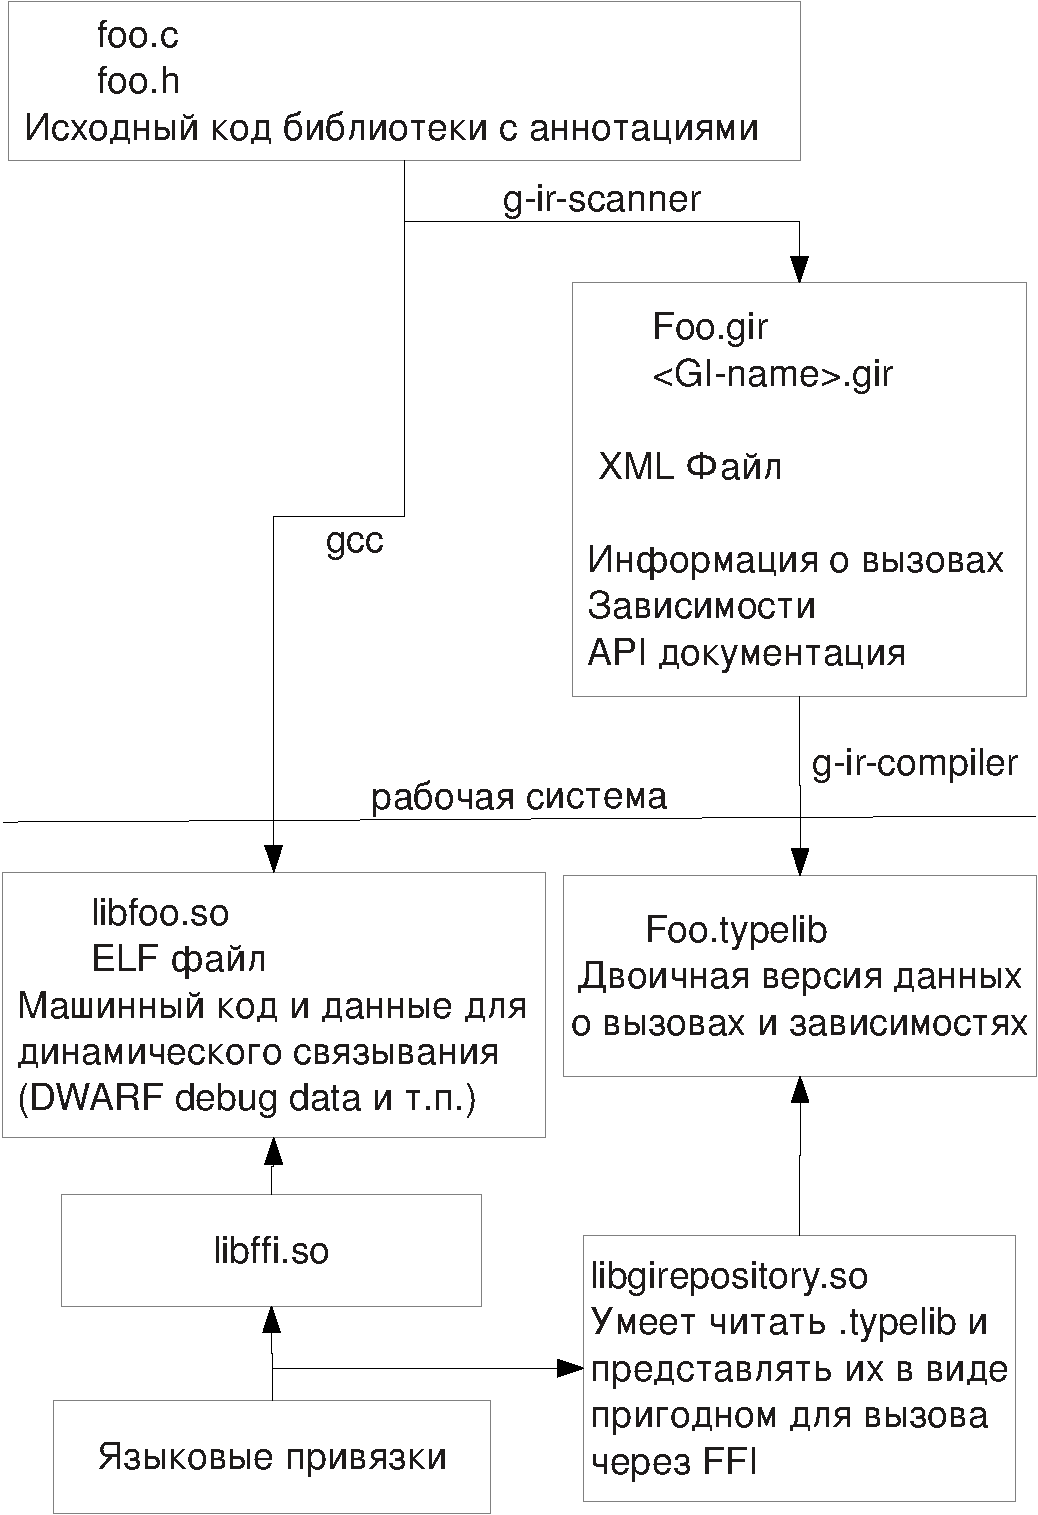
\includegraphics[width=10cm]{103_2012_antono-crop}
  \label{fig:Antono1}
\end{figure}

\subsection*{Примеры использования}

Я создал репозиторий \cite{Antono2} с примерами использования библиотеки,
базирующейся на GObject, через автоматические привязки для разных языков.

Рассмотрим пример, использующий язык Vala для создания библиотеки и
обращения к этой библиотеке из Ruby:

\begin{verbatim}
namespace ValaObject {
	public void say_hello_to(string lang)
	{
		print(@"I love You, $lang!!!\n");
		print("-- Vala\n\n");
	}

	public class ValaClass : Object {
		public string name = "Vala Class";

		public string append_to_name(string suffix) {
			return "%s %s".printf(name, suffix);
		}
	}
}
\end{verbatim}

Ruby использует метаданные из GIR через библиотеку gir\_ffi:

\begin{verbatim}
require 'gir_ffi'

GirFFI.setup(:ValaObject) # Создание объекта

ValaObject.say_hello_to('Ruby')

class MyValaClass < ValaObject::ValaClass
  def append_to_name(suffix)
    super + ' (subclassed) ' + suffix
  end
end

instance = MyValaClass.new
puts instance.append_to_name("called from Ruby")
\end{verbatim}

\subsection*{Существующие привязки}

Список существующих привязок для GObject Introspection выглядит следующим образом:

\begin{itemize}
  \item \url{https://live.gnome.org/Vala}{Vala} "--- Родная поддержка GIR.
  \item \url{https://live.gnome.org/Genie}{Genie} "--- Родная подержка GIR.
  \item \url{https://live.gnome.org/PyGObject}{PyGObject} "--- привязки для Python
  \item \url{https://live.gnome.org/Gjs}{Gjs} "--- Javascript (spidermonkey)
  \item \url{https://live.gnome.org/Seed}{Seed} "--- Javascript (JSCore, WebKit JS engine)
  \item \url{https://github.com/creationix/node-gir}{node-gir} "--- Node.js (V8 Engine)
  \item \url{https://github.com/mvz/ruby-gir-ffi/wiki}{ruby-gir-ffi} "--- Ruby
  \item \url{https://github.com/indeyets/gobject-for-php}{gobject-for-php} "--- PHP
  \item \url{http://oproj.tuxfamily.org/wiki/doku.php?id=lgob}{lgob} "--- Lua (этап компиляции)
  \item \url{https://github.com/pavouk/lgi}{lgi} "--- Lua (этап исполнения)
  \item \url{https://live.gnome.org/GTK2-Perl/Introspection}{GTK2-Perl/Introspection} "--- привязки для Perl
  \item \url{http://gitorious.org/guile-gir}{guile-gir} "--- Scheme (guile)
  \item \url{http://live.gnome.org/sbank}{sbank} "--- Scheme (Ikarus, Ypsilon)
  \item \url{https://live.gnome.org/JGIR}{JGIR} "--- Java/JVM (этап компиляции, через typelib)
  \item \url{https://live.gnome.org/GObjectIntrospection/GObjectConsume}{GObjectIntrospection/GObjectConsume} "--- C++, Qt (этап компиляции)
  \item \url{https://github.com/ex-rzr/factor-gir}{factor-gir} "--- Factor
  \item \url{https://github.com/indeyets/gobject-for-php}{gogobject} "--- Go (этап компиляции)
  \item \url{https://github.com/andy128k/cl-gobject-introspection}{cl-gobject-introspection} "--- Common Lisp
  \item \url{http://bazaar.launchpad.net/~scymtym/+junk/cl-gir/files}{cl-gir} "--- GIR for Common Lisp (в процессе)
  \item \url{http://www.haskell.org/haskellwiki/GObjectIntrospection}{haskel-gi} "--- Haskell (в процессе)
  \item \url{https://github.com/alanmcgovern/mono-introspect}{mono-introspect} "--- Mono
  \item \url{http://git.ocamlcore.org/cgi-bin/gitweb.cgi?p=ocaml-gir/ocaml-gir.git}{ocaml-gir} "--- Ocaml (этап компиляции)
  \item \url{http://wiki.freepascal.org/gir2pascal}{gir2pascal} "--- Pascal
\end{itemize}



\begin{thebibliography}{9}

\bibitem{Antono1} GTK+ Language Bindings. \url{http://www.gtk.org/language-bindings.php}

\bibitem{Antono2} GObject for your favorite language. \url{https://github.com/antono/vala-object}

\end{thebibliography}

\end{document}




